\documentclass[a4paper, titlepage, openany, oneside, 12pt]{book}
\usepackage{fancyvrb}
\usepackage[pdftex]{graphicx}
\usepackage{pfc}
\usepackage{float}
\usepackage{listings}                   % para formatar cdigo-fonte (ex. em Java)

\newcommand{\cod}[1]{{\renewcommand{\baselinestretch}{1}\scriptsize\VerbatimInput[xleftmargin=8mm,numbers=left,obeytabs=true]{cod/#1}}}

%===== C�digos Fonte =====
\newenvironment{codeverbatim}{\VerbatimEnvironment \small
   \begin{Verbatim}[xleftmargin=20mm]}
   {\end{Verbatim}}
%=======
\floatstyle{plain}  % tipos: plain, boxed, ruled
\newfloat{codigo}{tbp}{lop}[section] % numera os captions com  n�mero de se��o.
\floatname{codigo}{C�digo}
% nome para ser usado no sum�rio
\newcommand{\listofcodename}{Lista de C�digos}
%=========================

% ---------------------------------------------------------------------------- %
% Opes de listing usados para o cdigo fonte
% Ref: http://en.wikibooks.org/wiki/LaTeX/Packages/Listings
\lstset{ %
language=Java,                  % choose the language of the code
basicstyle=\footnotesize,
basicstyle=\footnotesize,       % the size of the fonts that are used for the code
numbers=left,                   % where to put the line-numbers
numberstyle=\footnotesize,      % the size of the fonts that are used for the line-numbers
stepnumber=1,                   % the step between two line-numbers. If it's 1 each line will be numbered
numbersep=5pt,       % the size of the fonts that are used for the code
showspaces=false,               % show spaces adding particular underscores
showstringspaces=false,         % underline spaces within strings
showtabs=false,                 % show tabs within strings adding particular underscores
frame=single,	                % adds a frame around the code
framerule=0.6pt,
tabsize=2,	                    % sets default tabsize to 2 spaces
captionpos=b,                   % sets the caption-position to bottom
breaklines=true,                % sets automatic line breaking
breakatwhitespace=false,        % sets if automatic breaks should only happen at whitespace
escapeinside={\%*}{*)},         % if you want to add a comment within your code
extendedchars=true,
xleftmargin=10pt,
xrightmargin=10pt,
framexleftmargin=10pt,
framexrightmargin=10pt
}

%--------------------------------------------------------%

\begin{document}

%%%%%%%%%%%%%%%%%%%%%%%%%%%%%%%%%%%%%%%%%%%%%%%%%%%%%%%%%%%%%%%%%%%%%%
%%%                       DADOS PESSOAIS                           %%%
%%%%%%%%%%%%%%%%%%%%%%%%%%%%%%%%%%%%%%%%%%%%%%%%%%%%%%%%%%%%%%%%%%%%%%

\titulo{Estudo de um compilador sob a perspectiva de um sistema online de programa��o}
\area{Compiladores}
\pchaveA{Compilador} \pchaveB{Sistemas Web}
\pchaveC{Linguagem de Programa��o} \autor{N�lio Carneiro J�nior}
\autorsobrenomenome{Carneiro, N�lio}
\autorsobrenomeiniciais{Carneiro, N�lio}
\orientador{Ms. Thiago Jabur Bittar} \avaliadorA{Professor 1}
\avaliadorB{Professor 2} \ano{2011} \mes{Junho}

%%%%%%%%%%%%%%%%%%%%%%%%%%%%%%%%%%%%%%%%%%%%%%%%%%%%%%%%%%%%%%%%%%%%%%
%%%                     ELABORA DOCUMENTO                          %%%
%%%%%%%%%%%%%%%%%%%%%%%%%%%%%%%%%%%%%%%%%%%%%%%%%%%%%%%%%%%%%%%%%%%%%%
\pagestyle{empty}
\fazcapa
\newpage
\folharosto
\newpage
\fichacatalografica
\newpage
\paginaassinatura
\newpage
\vfill

\begin{flushright}
\begin{minipage}[b]{10cm}
\it{Dedico este trabalho}
\end{minipage}
\end{flushright}

\newpage
\vfill

\centro{AGRADECIMENTOS}


Por fim, agrade�o a todos que de forma direta ou indireta que
cotribu�ram para a minha forma��o.

\newpage

\begin{flushright}
\begin{minipage}[b]{10cm}
\it{``Os desafios.}
\end{minipage}

{\it{Sulamita}}
\end{flushright}

\newpage

%\paginaresumo % escreva seu resumo no arquivo resumo.tex

\pagestyle{plain}

\pagenumbering{roman}
\tableofcontents
\listoffigures
%\listoftables
%\listofalgorithms %requer \usepackage{algorithm} \usepackage{algorithmic}
%\listof{codigo}{\listofcodename}  % Lista de C�digos
\newpage
\pagenumbering{arabic}

%%%%%%%%%%%%%%%%%%%%%%%%%%%%%%%%%%
%%% INCLUA AQUI SEUS CAP�TULOS %%%
%%%%%%%%%%%%%%%%%%%%%%%%%%%%%%%%%%


\newpage
\addcontentsline{toc}{chapter}{Introdu��o}
\chapter*{Introdu��o}
� evidente o crescente n�mero de usu�rios conectados � internet ao longo do tempo. 
Percebe-se tamb�m que esses usu�rios est�o cada vez mais necessitados de que suas ferramentas, 
antes usadas em seus desktops, fiquem dispon�veis online, de prontid�o, sempre que se fizer 
necess�rio, mesmo estando conectados longe de casa. Fez-se ent�o necess�rio que o desenvolvimento
de softwares caminhasse neste mesmo sentido.

Um aspecto interessante desse processo a ser analisado s�o as aplica��es que dependem de um compilador, 
ou seja, programas que quando instalados na m�quina sempre fazem uso de um compilador ou ent�o, s�o eles
 mesmos, compiladores. Um exemplo desse tipo de software seria um compilador para Portugol. 
Como iria se comportar tal compilador ao ser usado na internet? Como se daria a implementa��o deste 
compilador? Quais aspectos a serem tratados? E como seria o sistema na web que necessitasse desse compilador?

O objetivo principal deste trabalho � analisar o comportamento de um compilador feito para a 
linguagem Portugol, trabalhando sob um sistema de progama��o na Web. A proposta � fazer
um estudo detalhado da implementa��o desse compilador, tendo assim uma base s�lida para o desenvolvimento
do mesmo, visando na pr�tica tecer conclus�es � respeito das t�cnicas utilizadas.

Este trabalho tamb�m tem como objetivo desenvolver uma aplica��o Web que ir� utilizar o compilador.
A aplica��o � um editor o qual o usu�rio faz seus programas em Portugol, tendo de imediato a 
resposta do compilador. A inten��o � analisar como ir� se comportar o compilador, bem como, 
verificar a viabilidade de uso de tal aplica��o, ao se implementar utilizando as t�cnicas descritas 
ao longo deste trabalho. A aplica��o tem um car�ter educativo, no qual o usu�rio faz programas e, 
ele e seus trabalhos, podem ser acompanhados por um instrutor, visando assim verificar os passos 
realizados pelo usu�rio, bem como a maneira pela qual o compilador tem sido usado.

Uma grande vantagem da cria��o de tal sistema ser� o fato dele poder ser acessado de qualquer lugar e qualquer
m�quina, independente do sistema operacional, bastando apenas um navegador. Como exemplo, podemos citar uma faculdade
que possui bastantes m�quinas e algumas inclusives com sistemas operacionais diferentes. Outro fator s�o as
atualiza��es. Tendo um compilador online, basta atualizar em um s� lugar e a mudan�a ocorrer� para todos, diferente
de um compilador instalado em m�quinas locais.

No cap�tulo 1 s�o abordados os conceitos de compiladores, as t�cnicas utilizadas na cria��o
 do compilador e como se dar� o seu funcionamento diante uma aplica��o Web.

No cap�tulo 2 � feita uma apresenta��o da linguagem do compilador: o Portugol. Suas caracter�sticas
 e o embasamento para a cria��o do compilador baseado nesta linguagem tamb�m far� parte deste cap�tulo

No cap�tulo 3 pode-se observar um levantamento sobre o estado da arte dos compiladores e como tem sido
 o uso destes em aplica��es na Web. Neste tamb�m irei citar casos em que editores/compiladores foram 
colocados na Web.

No cap�tulo 4 � discorrido sobre a metodologia proposta para o desenvolvimento do prot�tipo de 
editor/compilador Web.

No cap�tulo 5 � abordado todo o processo de testes, al�m de ser realizado uma an�lise dos resultados. 
Por fim h� uma conclus�o do trabalho realizado, levantando os objetivos alcan�ados, pontos positivos, 
pontos negativos, dificuldades e trabalhos futuros.

Ainda � poss�vel encontrar o c�digo fonte do compilador e da aplica��o Web criada, al�m de toda a documenta��o
 de testes elaborada no ap�ndice desta monografia.

\chapter{Compiladores}
\section{Introdu��o}

Criado por volta dos anos 50, o nome Compilador se refere ao processo 
de composi��o de um programa atrav�s da reuni�o de v�rias rotinas de bibliotecas. 
O processo de tradu��o (de uma linguagem fonte para uma linguagem objeto), 
considerado hoje a fun��o central de um compilador, era ent�o conhecido como 
programa��o autom�tica[Rangel, 1999]

Definido em [AHO, 1995], um compilador � um programa que l� outro programa 
escrito em uma linguagem --- a linguagem de origem --- e o traduz em um programa 
equivalente em outra linguagem --- a linguagem de destino. Como uma importante 
parte no processo de tradu��o, o compilador reporta ao seu usu�rio a presen�a 
de erros no programa origem.

Ao longo dos anos 50, os compiladores foram considerados programas notoriamente
dif�ceis de escrever. O primeiro compilador Fortran, por exemplo, consumiu
18-homens ano para implementar[Backus, 1957]. Desde ent�o, foram descobertas
t�cnicas sistem�ticas para o tratamento de muitas das mais importantes
tarefas desenvolvidas por um compilador.

A variedade de compiladores nos dias de hoje � muito grande. Existem in�meras
linguagens fontes, as quais poderiam ser citadas em v�rias p�ginas deste trabalho. Isso
se deve principalmente ao fato de que com o aumento do uso dos computadores, aumentou
tamb�m, as necessidades de cada indiv�duo, sendo estas espec�ficas, exigindo por sua vez
linguagens de programa��o diferentes. Este processo --- juntamente com
a evolu��o da tecnologia de desenvolvimento de compiladores --- levou � cria��o de v�rias
t�cnicas diferentes para a constru��o de um compilador, ou seja, passou a existir
diferentes maneiras de se implementar um compilador. No entanto, a despeito dessa
aparente complexidade, as tarefas b�sicas que qualquer compilador precisa realizar
s�o essencialmente as mesmas.

A grande maioria dos compiladores de hoje fazem uso da t�cnica chamada: \textit{tradu��o
dirigida pela sintaxe}. Nesta t�cnica as regras de contru��o do programa fonte s�o utilizadas
para guiar todo o processo de compila��o.
Algumas das t�cnicas mais antigas utilizadas na contru��o dos primeiros compiladores (da
linguagem Fortran) pode ser obtido em [Rosen, 1967].

\section{Modelo de Compila��o de An�lise e S�ntese}

Ainda segundo [Rangel, 1999], existem duas tarefas triviais a serem executadas 
por um compilador nesse processo de tradu��o:

\begin{itemize}
 \item \textit{an�lise}, em que o texto de entrada (na linguagem fonte) � 
examinado, verificado e compreendido
 \item \textit{s�ntese}, ou \textit{gera��o de c�digo}, em que o texto de sa�da 
(na linguagem objeto) � gerado, de forma a corresponder ao texto de entrada.
\end{itemize}

Em [Aho, 1995], \textit{an�lise} � colocada como uma tarefa que divide o programa
fonte nas partes constituintes e cria uma representa��o intermedi�ria do mesmo. E
\textit{s�ntese} constr�i o programa alvo desejado, a partir da representa��o intermedi�ria.

Geralmente, pensamos nessas tarefas como fases que ocorram durante o processo de
 compila��o. No entanto, n�o se faz totalmente necess�rio que a an�lise de todo 
o programa seja realizada antes que o primeiro trecho de c�digo objeto seja gerado. 
Ou seja, estas duas fases podem ser intercaladas. Por exemplo, o compilador pode 
analisar cada comando do programa de entrada e ent�o gerar de imediato o c�digo 
de sa�da correspondente ao respectivo comando. Ou ainda, o compilador pode esperar 
pelo fim da an�lise de cada bloco de comando --- ou unidade de rotina 
(rotina, procedimentos, fun��es) --- para ent�o gerar o c�digo correspondente ao bloco.
Para aproveitar melhor a mem�ria durante a execu��o, compiladores costumavam ser divididos
em v�rias etapas, executados em sequ�ncia. Cada etapa constitui uma parte do processo de
tradu��o, transformando assim o c�digo fonte em alguma estrutura intermedi�ria adequada,
cada vez mais pr�xima do c�digo objeto final.

� natural que a an�lise retorne como resultado uma representa��o do programa fonte que
contenha informa��o necess�ria para a gera��o do programa objeto que o corresponda.
Quase sempre, essa representa��o (conhecida como \textit{representa��o intermedi�ria}[Rangel, 1999])
tem como complemento tabelas que cont�m informa��es adicionais sobre o programa fonte.
Pode ter casos em que a representa��o intermedi�ria toma a forma de um programa em uma
\textit{linguagem intermedi�ria}, deixando assim mais f�cil a tradu��o para a linguagem
objeto desejada.

N�o importando a maneira pela qual se toma a representa��o intermedi�ria, ela tem de conter
necessariamente toda a informa��o para a gera��o do c�digo objeto. Uma das caracter�sticas da
representa��o intermedi�ria � que as estruturas de dados implementadas devem dar garantia de 
acesso eficiente as informa��es.

Imagem - Rangel[1999]

Segundo [Rangel, 1999], uma das formas mais comuns de tabela utilizada nessa representa��o
intermedi�ria � a \textit{tabela de s�mbolos}, em que se guarda para cada identificador(\textit{s�mbolo})
usado no programa as informa��es correspondentes.

H� tamb�m um modelo poss�vel em [Ullman, 1977], o qual se faz a separa��o total entre o \textit{front-end},
encarregado da fase de an�lise, e o \textit{back-end}, encarregado pela gera��o de c�digo.
Com isso tem-se que:

\begin{itemize}
 \item front-end e back-end se comunicam apenas da representa��o intermedi�ria;
 \item o front-end depende exclusivamente da linguagem fonte
 \item o back-end depende exclusivamente da linguagem objeto.
\end{itemize}

Essa id�ia tem como objetivo simplificar a implementa��o de diferentes linguagens de programa��o para
diferentes m�quinas. Basta-se ent�o escrever um front-end para cada linguagem e um back-end para cada
m�quina. Ou seja, se deseja implementar \textit{x} linguagens para \textit{y} m�quinas, precisa-se fazer
\textit{x} front-ends e \textit{y} back-ends. Este esquema se torna mais f�cil de aplicar quando h�
semelhan�a entre as m�quinas e o mesmo acontece com as linguagens.

\section{An�lise}

� normal associar a \textit{sintaxe} a id�ia de forma, em oposi��o a \textit{sem�ntica} que se
associa a significado, conte�do. Tem-se ent�o que a sintaxe de uma linguagem de programa��o
deve descrever todos os aspectos relativos � forma de constru��o de programas corretos na linguagem,
enquanto a sem�ntica deve descrever o que acontece quando o programa � executado. Portanto, toda
an�lise est� relacionada com sintaxe, e a sem�ntica deveria corresponder apenas � gera��o de c�digo,
que deve preservar o significado do programa fonte, contruindo um programa objeto com o mesmo
significado[Rangel, 1999]

� necess�rio ressaltar uma diferen�a existente entre a teoria e a pr�tica. Quando falamos em teoria,
somente os programas corretos pertencem � linguagem, n�o havendo interesse nos programas incorretos.
O fato � que um programa ou � da linguagem (est� correto) ou n�o � da linguagem (est� incorreto).
No entanto, em se tratando de pr�tica, no momento em que decide-se que um programa est� incorreto,
um bom compilador dever� ser capaz de avisar sobre tal erro e de alguma forma, ajudar o usu�rio
a corrig�-lo. Se faz necess�rio que o tratamento de erros inclua mensagens informativas e
uma recupera��o, para que a an�lise possa continuar e assim outros erros sejam sinalizados.

Em [AHO, 1995] vemos que a an�lise se constitui em 3 fases:

\begin{itemize}
 \item \textit{An�lise Linear - An�lise L�xica}, na qual um fluxo de caracteres constituindo um programa � lido
da esquerda para a direita e agrupado em \textit{tokens}, que s�o sequ�ncias de caracteres tendo
um significado coletivo.
 \item \textit{An�lise Hier�rquica - An�lise Sint�tica}, na qual os caracteres ou \textit{tokens} s�o agrupados
hierarquicamente em cole��es aninhadas com significado coletivo.
 \item \textit{An�lise Sem�ntica}, na qual certas verifica��es s�o realizadas a fim de se
assegurar que os componentes de um programa se combinam de forma significativa.
\end{itemize}

Sabe-se da possibilidade de total representa��o da sintaxe de uma linguagem de programa��o
atrav�s de uma gram�tica sens�vel ao contexto [Wijngaarden, 1969]. No entanto, n�o
h� algoritmos pr�ticos para tratar estas gram�ticas, fazendo com que haja prefer�ncia
em usar gram�ticas livres de contexto. Sendo assim, fica claro que a separa��o entre
an�lise sint�tica e an�lise sem�ntica � dependente da implementa��o.

Sendo assim, a an�lise l�xica tem como finalidade separar e identificar os elementos
componentes do programa fonte, o qual estes geralmente, s�o especificados atrav�s de
express�es regulares. A an�lise sint�tica deve reconhecer a estrutura global do programa,
descrita atrav�s de gram�ticas livre de contexto. A an�lise sem�ntica se encarrega da
verifica��o das regras restantes. Essas regras tratam quase sempre da verifica��o de
que os objetos s�o usados no programa da maneira prevista em suas declara��es, por exemplo
verificando que n�o h� erros de tipos [Rangel, 1999].

N�o h� ainda um modelo matem�tico que se adeque inteiramente na fun��o de descrever o que deve
ser verificado durante a an�lise sem�ntica, ao contr�rio do que ocorre nas outras duas fases. No
entanto, alguns mecanismos, como gram�tica de atributos, tem sido utilizados com sucesso no processo
de simplifica��o da constru��o de analisadores sem�nticos.

\subsection{An�lise L�xica}

Segundo [AHO, 1995], o analisador l�xico � a primeira fase de um compilador. Sua tarefa principal �
a de ler os caracteres de entrada e produzir uma sequ�ncia de \textit{tokens} que o \textit{parser}
utiliza para a an�lise sint�tica. Essa intera��o � comumente implementada fazendo com que o analisador
l�xico seja uma subrotina do \textit{parser}. Ao receber do \textit{parser} um comando 'obter o pr�ximo
\textit{token}', o analisador l�xico l� os caracteres de entrada at� que possa identificar o pr�ximo
\textit{token}.

J� em [Ullman, 1977], vemos que a an�lise l�xica � respons�vel por separar e identificar os elementos componentes
do c�digo fonte. A an�lise l�xica tamb�m elimina os elementos considerados 'decorativos' ou mesmo desnecess�rios
para este processo, tais como espa�os em branco, marcas de formata��o de texto e coment�rios.

Em [Rangel, 1995] temos o seguinte exemplo em Pascal:

\begin{lstlisting}
 if x > 0 then        {x e' positivo}
     modx := x
 else                 {x e' negativo}
     modx := (-x)
\end{lstlisting}

Ap�s a an�lise l�xica, a sequ�ncia de \textit{tokens} identificadas �:

\begin{center}
\begin{tabular}{cc}
\hline
\textbf{Tipo do \textit{token}} & \textbf{Valor do \textit{token}}\\
\hline
palavra reservada if & if\\
\hline
identificador x & x\\
\hline
operador maior & >\\
\hline
literal num�rico & 0\\
\hline
palavra reservada then & then\\
\hline
identificador & modx\\
\hline
operador de atribui��o & :=\\
\hline
identificador & x\\
\hline
palavra reservada else & else\\
\hline
identificador & modx\\
\hline
operador de atribui��o & :=\\
\hline
delimitador abre par�ntese & (\\
\hline
operador menos un�rio & -\\
\hline
identificador & x\\
\hline
delimitador fecha parenteses & )\\
\hline
\end{tabular}
\end{center}

Normalmente os tipos dos \textit{tokens}(na primeira coluna) s�o representados por valores de um tipo de enumera��o
ou por c�digos num�ricos apropriados.

O que vemos na grande maioria das vezes � que a implementa��o de um analisador l�xico � baseada em um aut�mato
finito capaz de reconhecer as diversas constru��es.

\chapter{Portugol}
\section{Introdu��o}

O Portugol como linguagem n�o � t�o bem definida, ficando muito mais sujeita a uma
linguagem de aprendizado, voltada para o ensino e n�o para projetos de
grande porte. Algumas vezes � somente uma tradu��o simplificada de Pascal
para o portugu�s.

O Portugol aqui definido ser� baseado em \cite{Farrer1999}. O Livro utilizado para
o estudo de algoritmos e de introdu��o a programa��o, � perfeito para
este trabalho. O compilador desenvolvido, bem como o sistema Web, visa estudar
como o processo de compila��o online se dar�, sendo necess�rio uma linguagem
simples que n�o tome o foco do objetivo principal.

Nas se��es subsequentes veremos como o portugol foi proposto para este compilador.
Suas caracter�sticas, sua sintaxe e a estrutura da linguagem.

\section{Estrutura da Linguagem}

\subsection{Coment�rios}

Mais de uma forma de comentar o c�digo ser� aceito, estimulando o seu uso em todo o
c�digo. O // usado em linguagens como C e Java e tamb�m a \# (cerquilha), utilizada em 
linguagens como o Ruby s�o aceitos como coment�rios de uma s� linha. Os {} (colchetes)
s�o a �nica forma aceita de coment�rios para v�rias linhas ou coment�rios de bloco.

\subsection{Tipos b�sicos}

Os tipos b�sicos s�o simples e restritos, pois visam o ensino da l�gica de programa��o.
Isso promove tamb�m a independ�ncia de linguagem e de m�quina.

\subsubsection{Num�rico}

O tipo num�rico resume todos os tipos para o c�lculo aritm�tico. N�o existe distin��o entre
n�meros inteiros ou n�meros reais (ponto flutuante). Caso haja a necessidade de que algum
algoritmo utilize uma propriedade espec�fica de algum destes tipos, dever� esta ser obtida
atrav�s de fun��es. A v�rgula � o s�mbolo utilizado para a separa��o da parte decimal.
N�o se escrevem os separadores de milhar.

\subsubsection{Literal}

Este tipo � respons�vel por armazenar sequ�ncias de letras e s�mbolos --- em muitas
linguagens � o tipo \textit{String}. 

\subsubsection{L�gico}

Respons�vel pelo armazenamento das constantes verdadeiro e falso. Este tipo � muito
importante em projetos de linguagens de programa��o, visto que ele � bastante
utilizado, sendo o tipo de retorno de v�rias opera��es.

\subsubsection{Vetores e Matrizes}

� permitida a cria��o de vetores e matrizes de quaisquer tipos b�sicos. As opera��es realizadas
com matrizes e vetores dever�o ser realizadas de forma condizente com a linguagem Portugol.
As opera��es b�sicas deste tipo seguem as mesmas permitidas em seus tipos b�sicos. A palavra-chave
\textit{matriz} � reservada para este tipo. O n�mero inicial dos �ndices � sempre 1.

Exemplo:

 
\begin{lstlisting}
a matriz num�rico[30]  // Cria uma matriz 30x1
b matriz l�gico[3][3]  // Cria uma matriz 3x3
 
\end{lstlisting}


\subsubsection{Registros}

� sempre definido pela palavra reservada \textbf{registro}. Representa um bloco composto
por declara��es de vari�veis. Se encerra com a palavra \textbf{fimregistro}.

Exemplo:

\begin{lstlisting}
 registro
   num1, num2 num�rico
   estaPresente l�gico
   endereco literal
 fimregistro
\end{lstlisting}

\subsection{Vari�veis e Identificadores}

As vari�veis s�o parte importante de uma linguagem. Qualquer identificador, sendo este v�lido, tem
como primeiro s�mbolo uma letra. N�meros e \_ (sublinha) s�o aceitos ap�s o primeiro caractere. O
tamanho m�ximo v�lido � definido em 32 caracteres.

� necess�rio lembrar que alguns s�mbolos, normalmente ignorados ou proibidos em outras linguagens,
s�o aceitos em Portugol. S�mbolos estes presentes na l�ngua portuguesa, como por exemplo, os acentos:
�, �, �, �, �, ..., �.

Vale ressaltar da diferen�a existente entre vari�veis declaradas com acento e vari�veis sem acento.
Ou seja, a vari�vel 'p�' � diferente da vari�vel 'pe'.

\subsection{Declara��o de vari�veis}

N�o existe um local espec�fico para declara��o de vari�veis, mas fica a recomenda��o de que esta
seja feita no in�cio de uma se��o, seja o programa principal ou um procedimento/fun��o. A
palavra-chave \textbf{declare} ser� utilizada para declarar vari�veis em Portugol. � poss�vel
declarar vari�veis de mesmo tipo em uma mesma linha, nunca vari�veis de tipos diferentes.

Exemplo:

\begin{lstlisting}
 declare num1, num2, num3 num�rico
 declare palavra literal
 declare a, b, c l�gico
 declare r registro
		    dia, mes num�rico
		    nome literal
		    estaPresente l�gico
	   fimregistro
\end{lstlisting}

Exemplo de declara��o inv�lida:

\begin{lstlisting}
 declare num1 num�rico, palavra literal
\end{lstlisting}

A visibilidade de uma palavra segue o mesmo padr�o de outras conhecidas linguagens, ou seja, �
dependente do escopo a qual foi definida.

\subsection{Atribui��o}

A atribui��o de valores a uma vari�vel ser� denotada pelo s�mbolo '':=''. Ser� permitido 
apenas a atribui��o de um valor por vez. Uma atribui��o ser� v�lida quando possuir
um identificador v�lido do lado esquerdo e uma express�o v�lida e, do mesmo tipo, do
lado direito.

Exemplo:

\begin{lstlisting}
 declare num1, num2 num�rico
 declare palavra literal

 num1 := 3
 num2 := 1,5
 palavra := "Ol� Mundo"
\end{lstlisting}

\subsection{Operadores}

\subsubsection{Operadores Aritm�ticos}

Os operadores s�o:

\begin{center}
\textbf{Tabela 2.1 - Operadores Aritm�ticos}
\end{center}

\begin{center}
\begin{tabular}{cc}
\hline
\textbf{Opera��o} & \textbf{S�mbolo}\\
\hline
Adi��o & +\\
\hline
Subtra��o & -\\
\hline
Multiplica��o & *\\
\hline
Divis�o & /\\
\hline
\end{tabular}
\end{center}

\subsubsection{Operadores L�gicos}

Os Operadores s�o:

\begin{center}
\textbf{Tabela 2.2 - Operadores L�gicos}
\end{center}

\begin{center}
\begin{tabular}{cc}
\hline
\textbf{Opera��o} & \textbf{S�mbolo}\\
\hline
invers�o - n�o & n�o\\
\hline
jun��o & e\\
\hline
disjun��o & ou\\
\hline
\end{tabular}
\end{center}

\subsubsection{Operadores Relacionais}

Os Operadores s�o:

\begin{center}
\textbf{Tabela 2.3 - Operadores Relacionais}
\end{center}

\begin{center}
\begin{tabular}{cc}
\hline
\textbf{Opera��o} & \textbf{S�mbolo}\\
\hline
Igualdade & =\\
\hline
Maior & >\\
\hline
Menor & <\\
\hline
Maior ou Igual & >=\\
\hline
Menor ou Igual& <=\\
\hline
Diferen�a& != ou <>\\
\hline
\end{tabular}
\end{center}

\subsubsection{Operadores Relacionais}

Os Operadores s�o:

\begin{center}
\textbf{Tabela 2.4 - Operadores Literais}
\end{center}

\begin{center}
\begin{tabular}{cc}
\hline
\textbf{Opera��o} & \textbf{S�mbolo}\\
\hline
Concatena��o & +\\
\hline
Igualdade & =\\
\hline
Maior & >\\
\hline
Menor & <\\
\hline
Maior ou Igual & >=\\
\hline
Menor ou Igual& <=\\
\hline
Diferen�a& != ou <>\\
\hline
\end{tabular}
\end{center}

\subsection{Estrutura Sequencial}

O programa tem in�cio com a palavra \textbf{programa} e tem fim com a palavra
\textbf{fimprograma}. Caso queira importar outros m�dulos, estes devem ser feitos
atrav�s de comando, ap�s a declara��o do programa.

Em Portugol n�o se faz necess�ria a utiliza��o de algum s�mbolo especial ou visual
para marcar o fim de linha. Basta que o ''Retorno'' --- mais conhecido pela tecla
''ENTER'' --- seja pressionado. Este s�mbolo � definido na posi��o 13 da tabela
ASCII.

Qualquer que seja o s�mbolo ou comando declarado fora do escopo do programa, ser�
considerado erro. Fun��es e procedimentos devem ser declarados externamente e ent�o, 
importados pelo programa que necessite utiliz�-los. Isto far� com que se estimule
a modulariza��o de c�digo, bem como a cria��o de arquivos de menor tamanho e mais
f�ceis de entender.

\subsection{Estruturas Condicionais}

S�o definidas duas: \textbf{se} e o \textbf{caso}.

O \textbf{se} � utilizado quando se quer avaliar uma condi��o ou express�o
l�gica e retorna obrigatoriamente um valor l�gico. Conforme o retorno a
execu��o passa para o bloco \textbf{ent�o} --- caso seja verdadeiro ---
ou para o bloco \textbf{sen�o} --- caso seja falso.

� definido tamb�m em Portugol o \textbf{fiment�o} e o \textbf{sen�o}, respons�veis
pelo fechamento dos blocos \textbf{ent�o} e \textbf{sen�o} respectivamentes.

Exemplo:

\begin{lstlisting}
 se num1 > num2
     ent�o num1 = 1
     fiment�o
     sen�o num2 = 2
     fimsen�o
 fimse
\end{lstlisting}

A estrutura \textbf{caso} permite avaliar v�rios valores e admite v�riavel
dos tipos l�gicos, num�rico e literal.

\begin{lstlisting}
 caso tamanho
     10: i := 10
     11: i := 11
     12: i := 12
 fimcaso
\end{lstlisting}

\subsection{Estruturas de Repeti��o}

Tr�s estruturas s�o definidas em Portugol: \textbf{fa�a}, \textbf{enquanto}, \textbf{repita}.

O \textbf{fa�a} � similar ao \textit{for} de outras linguagens. Sua constru��o � demonstrada
abaixo:

\begin{lstlisting}
 fa�a i de 1 at� 10
     <instru��es>
 fimfa�a
\end{lstlisting}

O bloco acima ir� executar as instru��es dez vezes, incrementando o valor do ''i'' de 1 at� 10.
� recomend�vel como boas pr�ticas de programa��o que a v�riavel de controle --- no bloco
acima � o ''i'' --- n�o tenha seu valor alterado pelas instru��es internas. O valor do ''i'' �
incrementado em 1 sempre quando se chega ao ''fimfa�a''. O valor do ''i'' ap�s o ''fimfa�a'' �
igual ao valor m�ximo estipulado no in�cio, no caso 10.

O \textbf{enquanto} substitui o \textit{while} de outras linguagens de programa��o.
Exemplo:

\begin{lstlisting}
 enquanto num1 > num2
     <instru��es>
 fimenquanto
\end{lstlisting}

A estrutura de repeti��o \textbf{enquanto} executa o bloco de c�digo at� que a condi��o seja
falsa. Pode acontecer das instru��es nem serem executadas, caso a condi��o seja falsa logo
de in�cio.

A estrutura \textbf{repita} tem como caracter�stica o fato de ser b�sica. A verifica��o e a
interrup��o do bloco de c�digo � livre, sendo especificada pelo comando \textbf{interrompa}.
Veja:

\begin{lstlisting}
 repita
     <comandos>
     interrompa 
 fimrepita
\end{lstlisting}

Ap�s a leitura do interrompa, a execu��o do programa se dar� para o trecho de c�digo abaixo
do ''fimrepita''.

Como pode ser observado, a maioria das estruturas definidas s�o fechadas sempre utilizando o
''fim\textit{estrutura}''. A n�o utiliza��o de tal comando acarretar� em um erro de c�digo, 
podendo ser este l�xico ou sint�tico.

\subsection{Fun��es}

As fun��es aqui definidas seguem as mesmas regras de um programa, n�o podendo apenas importar m�dulos.

A declara��o de uma fun��o pode ser vista abaixo:

\begin{lstlisting}
 funcao soma(a numerico, b numerico)
     <comandos>
 fimfuncao
\end{lstlisting}

Assim como ocorre em outras linguagens de programa��o, as vari�veis declaradas em uma determinada fun��o
s�o internas a ela, possuindo assim escopo local.

Decidi por n�o utilizar uma estrutura do tipo procedimento - estrutura esta existente em outras linguagens -
pelo fato de simplificar o uso da linguagem, visto que ela se designa ao ensino de programa��o. O mesmo se
faz irrelevante neste trabalho, j� que a principal diferen�a entre uma fun��o e um procedimento � que a 
fun��o retorna um resultado.

\section{Conclus�o}

A linguagem Portugol � por sua pr�pria natureza simples. Na maioria das vezes em que � utilizada a finalidade � sempre
o aprendizado de programa��o de computadores. O Portugol utilizado para a constru��o deste trabalho tamb�m
tem a simplicidade em sua ess�ncia, no entanto, oferece as condi��es necess�rias para uma introdu��o a programa��o,
al�m de tamb�m atender ao prop�sito deste trabalho de final de curso.

� importante deixar claro que tomando como base este trabalho e a linguagem Portugol em si, � perfeitamente poss�vel
a cria��o de uma linguagem de programa��o mais poderosa e robusta que contenha uma estrutura muito mais complexa.
Ou ent�o � tamb�m poss�vel, a cria��o de uma DSL (Domain Specific Language), mas este seria um assunto para um 
outro projeto.

\chapter{Estado da Arte}
\section{Introdu��o}

A contru��o de compiladores, bem como o estudo do mesmo � algo antigo que acontece desde os prim�rdios da computa��o,
visto que desde sempre, fez-se necess�rio a comunica��o com as m�quinas e, a evolu��o dos compiladores e tamb�m
das linguagens de programa��o se baseou no estudo de t�cnicas que visavam melhorar tal comunica��o.

\section{Compiladores}


Conforme Knuth e Trabb  [KP80],  o termo compilador n�o era ainda utilizado nessa �poca. Na verdade falava-se
sobre programa��o autom�tica. No in�cio da programa��o em linguagem de m�quina foram desenvolvidas subrotinas de uso
comum para entrada e sa�da, para aritm�tica de ponto flutuante e fun��es  transcendentais. Junto com a id�ia de um
endere�amento realoc�vel - pois tais subrotinas seriam usadas em diferentes partes de um programa - foram criadas
rotinas de montagem para facilitar a tarefa de uso das subrotinas e de endere�amento relativo, id�ia desenvolvida por
Maurice V. Wilkes. Para isso foi inventada uma pseudo linguagem de m�quina. Uma rotina interpretativa iria processar
essas instru��es, emulando um computador hipot�tico  [Gol72] [Knu69]. Esse � o sentido do termo 'compilador' at�
aqui usado.

Nos prim�rdios dos computadores, programar era uma tarefa extremamente complicada e, de certa forma, extenuante.
Aos programadores era exigido um conhecimento detalhado das instru��es, registos e outros aspectos ligados com 
a unidade de processamento central (CPU) do computador onde era escrito o c�digo. Os programas consistiam numa s�rie
de instru��es num�ricas, denominadas por c�digo bin�rio. Posteriormente, desenvolveram-se algumas mnem�nicas que
resultaram no designado assembly. No per�odo entre 1954-1957 uma equipa de 13 programadores liderados por John Backus
desenvolveu uma das primeiras linguagens de alto n�vel para o computador IBM 704, o FORTRAN (FORmula TRANslation).
O objetivo deste projecto era produzir uma linguagem de f�cil interpreta��o, mas ao mesmo tempo, com uma efici�ncia
id�ntica � linguagem assembly [Abel, 2000].

A linguagem Fortran foi ao mesmo tempo revolucion�ria e inovadora. Os programadores libertaram-se assim da tarefa
extenuante de usar a linguagem assembler e passaram a ter oportunidade de se concentrar mais na resolu��o do problema.
Mas, talvez mais importante, foi o fato dos computadores passarem a ficar mais acess�veis a qualquer pessoa com
vontade de despender um esfor�o m�nimo para conhecer a linguagem Fortran. A partir dessa altura, j� n�o era preciso
ser um especialista em computadores para escrever programas para computador [Abel, 2000].

\chapter{Metodologia e An�lise do Prot�tipo Proposto}
\section{Introdu��o}

A cria��o de um compilador que realiza comunica��o com um navegador e realiza suas opera��es pela internet n�o
� t�o trivial de se fazer. Os compiladores tem como caracter�stica o fato de poderem demorar em uma determinada
compila��o, dependendo � claro da complexidade do algoritmo criado. J� o os navegadores de internet devem sempre
ter uma resposta imediata e r�pida na medida do poss�vel. Faz-se ent�o necess�rio que um compilador online deva manter
uma forma simples e limpa, para que facilite esse processo e seja ent�o vi�vel.

Este trabalho prop�e uma metodologia de compilador online, ou seja, um sistema que funcione em um navegador para a 
internet, compilando determinado trecho de c�digo e retornando o resultado para o usu�rio.

Basicamente o prot�tipo proposto � baseado em dois m�dulos principais, sendo eles o compilador e o sistema web.
Entre estes m�dulos existe portanto uma comunica��o, ou seja, o usu�rio acessa o sistema atrav�s da internet e
insere o seu c�digo. O sistema ent�o enviar� esse c�digo para a compila��o e ent�o, depois de compilado, o compilador
retorna a resposta para sistema web que apresentar� a mesma ao usu�rio.

O compilador foi criado utilizando a linguagem C++, visto que tal linguagem apresentou-se f�cil para a constru��o do
mesmo, al�m de possuir uma documenta��o vasta e ser bastante robusta. Para o processo de \textit{backend} foi utilizado
o NASM (Netwide Assembler)

\section{Compilador}

Como visto no cap�tulo 1, o compilador apresenta fases da compila��o, sendo elas a fase de an�lise e fase de s�ntese.
Cada uma destas fases s�o dividas em outras fases menores, sendo cada uma delas respons�veis por tarefas durante
todo o processo. Na fase de an�lise (tamb�m conhecida como \textit{frontend}) o processo se divide em tr�s, an�lise
l�xica, sint�tica e sem�ntica. Tais fases s�o respons�veis por identificar e informar a grande maioria dos erros por
parte do programador.

\subsection{An�lise L�xica}

A analise l�xica � o primeira m�dulo do \textit{frontend} de um compilador e basicamente este m�dulo � respons�vel por
receber um arquivo de entrada (programa fonte) e "quebr�-lo"em palavras conhecidas como tokens. Os analisadores
l�xicos tamb�m t�m a fun��o de descartar coisas que n�o ter�o import�ncia para a compila��o de um arquivo fonte
tais como: Espa�os em branco e coment�rios.

Como resultado um analisador l�xico verifica se um determinado c�digo � ou n�o v�lido de acordo com a gram�tica da 
linguagem regular descrita e gera uma lista de tokens que ser� repassada para os outros m�dulos do processo de 
compila��o A implementa��o de um analisador l�xico requer logicamente que a linguagem regular (a qual o analisador 
l�xico ira obedecer as regras) seja descrita formalmente e para isto faz-se necess�rio o uso de algumas estruturas de 
representa��o desta linguagem tais como as Express�es Regulares que ser� a base para a constru��o de um NFA(Aut�mato 
Finito N�o Determin�stico) e a partir deste NFA � contru�do um DFA (Aut�mato Finito Determin�stico) que representa a 
linguagem gramaticamente e � a base para a codifica��o usando uma linguagem de programa��o do analisador l�xico para
uma determinado linguagem regular.

Na figura 4.1 v�-se um NFA que tem como fun��o representar os operadores da linguagem.

\begin{figure}[!htb]
 \centering
 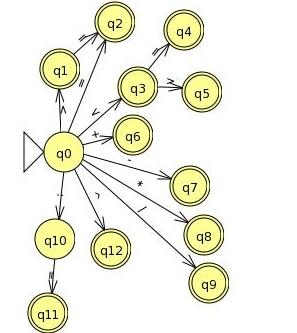
\includegraphics[scale=0.6]{imagens/fig10.jpg}
 \caption{NFA que representa as palavras reservadas da linguagem}
\end{figure}

J� na figura 4.2 temos um outro NFA, respons�vel por representar os coment�rios de linha.

\begin{figure}[!htb]
 \centering
 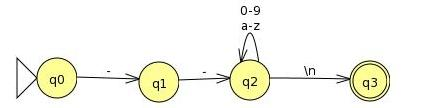
\includegraphics[scale=0.6]{imagens/fig11.jpg}
 \caption{NFA que representa os coment�rios de linha da linguagem}
\end{figure}

\subsection{An�lise Sint�tica}

Terminada a etapa de an�lise l�xica do nosso compilador, passamos agora para a segunda etapa de constru��o do mesmo: 
A an�lise Sint�tica. A etapa de an�lise sint�tica ou em ingl�s \textit{parser} recebe como entrada uma sequ�ncia de 
tokens do analisador l�xico e determina se a string pode ser gerada atrav�s da linguagem fonte. Para este compilador
foi criado um analisadore sint�tico do tipo \textit{LALR(1)}.

O analisador sint�tico preditivo � um algoritmo simples, capaz de fazer o \textit{parsing} de algumas linguagens. 
Neste tipo de analisador cada produ��o da linguagem fonte torna-se uma cl�usula em uma fun��o recursiva, tendo-se 
uma fun��o para cada n�o-terminal da produ��o. Como visto, cada fun��o relativa a um n�o-terminal precisa conter um
cl�usula para cada produ��o. Desta forma faz-se necess�rio saber escolher qual a produ��o mais apropriada para tal. 
Esta escolha � feita baseando-se no pr�ximo \textit{token}. E isto � feito atrav�s da \textit{predictive parsing table}.

A maioria das linguagens de programa��o � LALR(1), sendo esta t�cnica o tipo mais usado em geradores autom�ticos de
parsers, foi usado ent�o um analisador LALR(1) para a linguagem Portugol.

\subsection{An�lise Sem�ntica}

A an�lise sem�ntica � o ultimo m�dulo do \textit{frontend} de um compilador. Como j� foi visto a an�lise l�xica � 
respons�vel por quebrar a entrada em palavras conhecidas como \textit{tokens}. J� a an�lise sint�tica que � o segundo
m�dulo do \textit{frontend}, tem o objetivo de analisar a estrutura de frases de um programa e verificar tamb�m se 
determinada \textit{string} pode ser gerada pelas deriva��es da gram�tica em quest�o. Por fim a an�lise sint�tica
calcula o "significado" do programa realizando verifica��es de tipos e de declara��es e seus respectivos usos.o

\subsection{Backend}

Ap�s o processo de an�lise, o compilador gera c�digo em assembly para, ent�o, usar o NASM (Netwide Assembler) como
\textit{backend} para montar e criar um execut�vel v�lido. Consequentemente, n�o existe etapa de linkagem. A fase de
otimiza��o de c�digo tamb�m n�o foi implementada.

Para usar esse recurso, � nescess�rio que o NASM esteja instalado no sistema. Ele pode ser encontrado em [NASM, 2011].

\section{Sistema de Programa��o Web}

Como segundo m�dulo do prot�tipo proposto, tem-se a cria��o do Sistema de Programa��o Web que funciona com um editor de
programas e tamb�m realiza a comunica��o com o compilador.
O sistema tem como nome 'PortugOn'.

O sistema foi criado utilizando a linguagem de programa��o Ruby, juntamente com o framework Rails, pois � uma linguagem
de alto n�vel, capaz de realizar tarefas com menos linhas de c�digo que v�rias outras linguagens, sendo esta tamb�m
a linguagem a qual sou mais fluente. Foi escrito tamb�m c�digo JavaScript, para facilitar na intera��o com o usu�rio.
O banco de dados utilizado para a aplica��o foi o MySQL, por ser um banco popular, de f�cil integra��o com o Ruby
on Rails e tamb�m por ser de f�cil manuseio.

O PortugOn � dividido em telas, as quais cada uma tem as propriedades.
A princ�pio temos a tela inicial (como pode ser observado na figura 4.3), que tem como finalidade apresentar o sistema
atrav�s de algumas de suas caracter�sticas e tamb�m, cont�m um formul�rio de \textit{login} para que o usu�rio possa
realizar sua autentica��o no sistema. Caso o usu�rio ainda n�o tenha cadastro ele pode clicar em 'Cadastre-se' e a�
partir para uma outra tela, a de novo cadastro.

\begin{figure}[!htb]
 \centering
 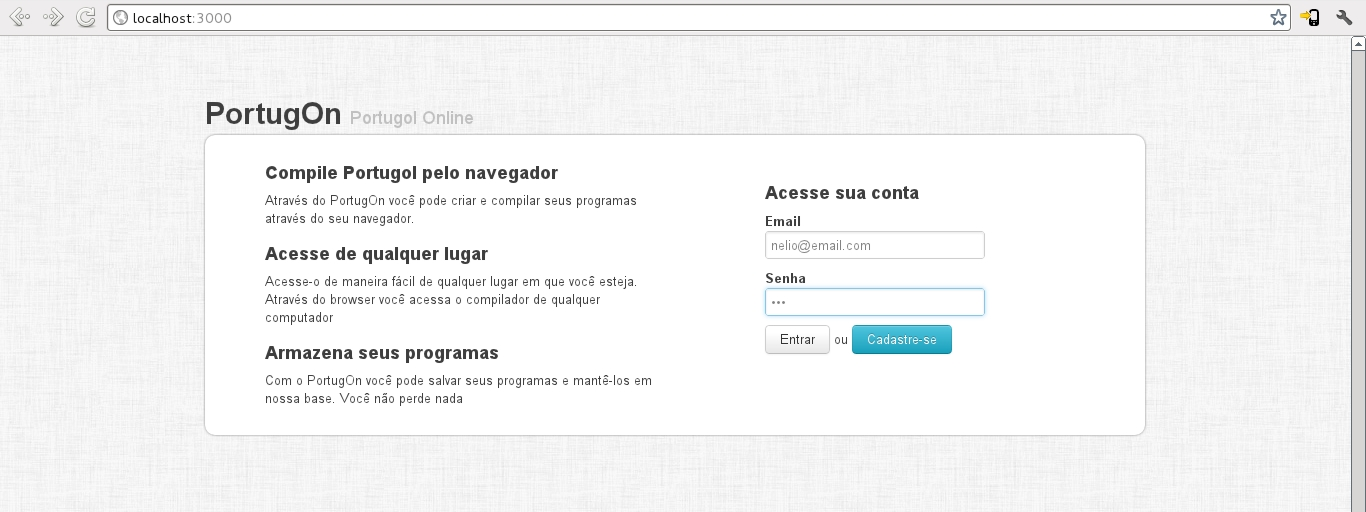
\includegraphics[scale=0.35]{imagens/tela1.jpg}
 \caption{P�gina inicial do sistema PortugOn}
\end{figure}

Se ent�o o usu�rio que acessar o sistema ainda n�o tiver cadastro, ele dever� realizar um novo. Ao clicar em
'Cadastre-se' na p�gina inicial, o usu�rio ir� para uma nova p�gina (figura 4.4). Nessa nova p�gina o usu�rio dever�
preencher todos os campos pedidos e ent�o clicar 'Cadastrar'. Ap�s isso o usu�rio ser� cadastrado no banco de dados e
poder� realizar o \textit{login}. Caso o usu�rio n�o queira realizar seu cadastro ele pode clicar em 'Cancelar' e
voltar � pagina inicial.

\begin{figure}[!htb]
 \centering
 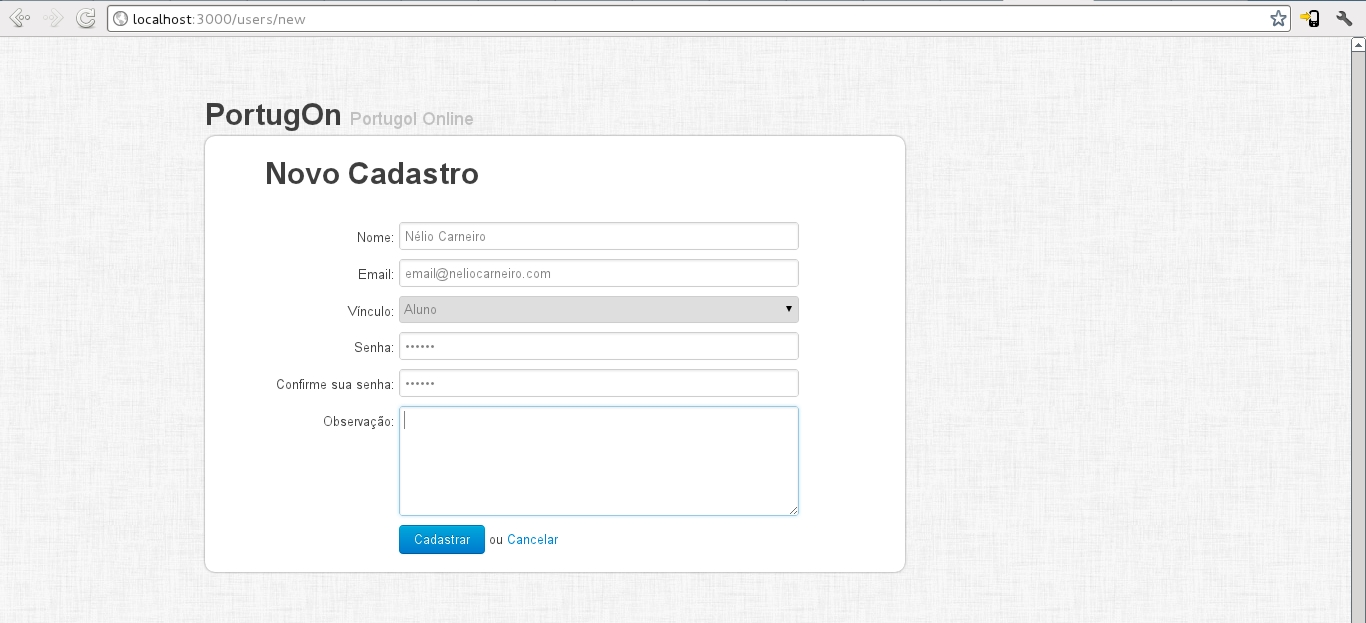
\includegraphics[scale=0.35]{imagens/tela2.jpg}
 \caption{P�gina de cadastro de usu�rio do sistema PortugOn}
\end{figure}

Ap�s o usu�rio efetuar o seu cadastro e entrar no sistema, ele ir� para a p�gina 'Home' (figura 4.5). Nesta p�gina ele ir� encontrar
um menu no topo, podendo navegar pelos links l� visualizados. Nessa mesma p�gina encontra-se o editor onde o usu�rio
deve entrar com o c�digo Portugol. Ao entrar com o c�digo do programa e clicar em 'Submit', o c�digo ser� compilado e
o retorno poder� ser observado na coluna ao lado, a coluna 'Resultado' (figura 4.6). O usu�rio receber� a mensagem
relacionada ao seu programa, se tudo correu bem, ser� uma mensagem de acerto, caso contr�rio o usu�rio receber� um
aviso de erro e a respectiva mensagem do compilador.

\begin{figure}[!htb]
 \centering
 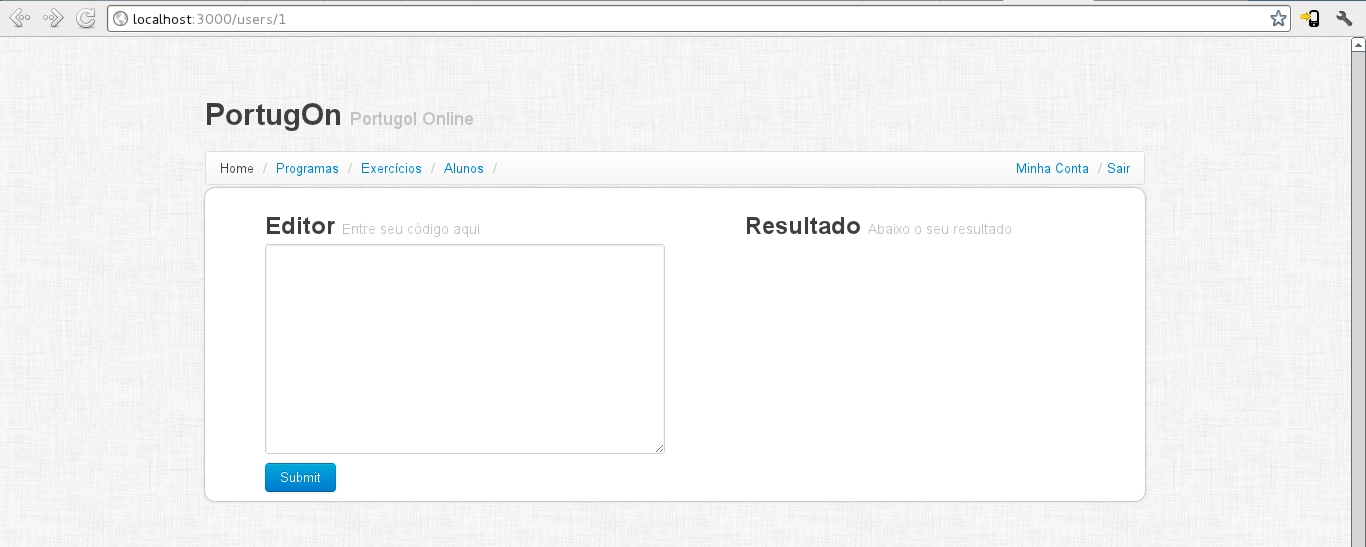
\includegraphics[scale=0.35]{imagens/tela3.jpg}
 \caption{Pagina Home do usu�rio do sistema PortugOn}
\end{figure}

\begin{figure}[!htb]
 \centering
 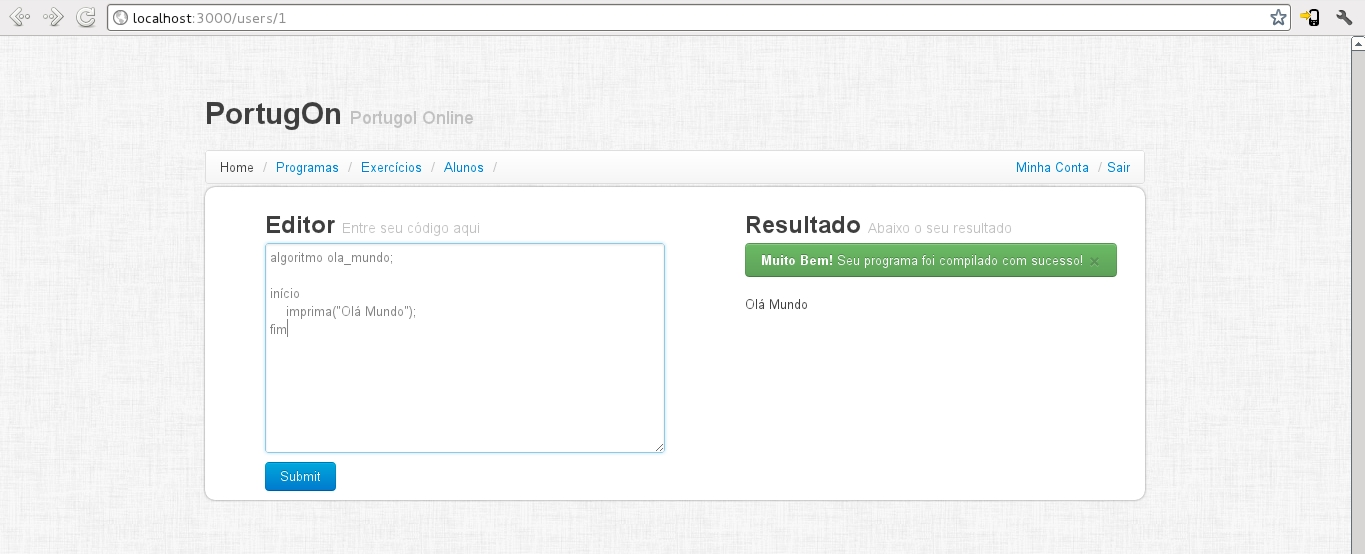
\includegraphics[scale=0.35]{imagens/tela4.jpg}
 \caption{P�gina Home do usu�rio, com c�digo compilado}
\end{figure}

Cada vez que o usu�rio compila determinado programa, este fica salvo no banco de dados. O usu�rio pode ent�o acessar
tais programas clicando no menu 'Programas' (figura 4.7). Essa tela mostra os programas j� feitos com a sua respectiva,
data, podendo o usu�rio editar o programa ou exclu�-lo.

\begin{figure}[!htb]
 \centering
 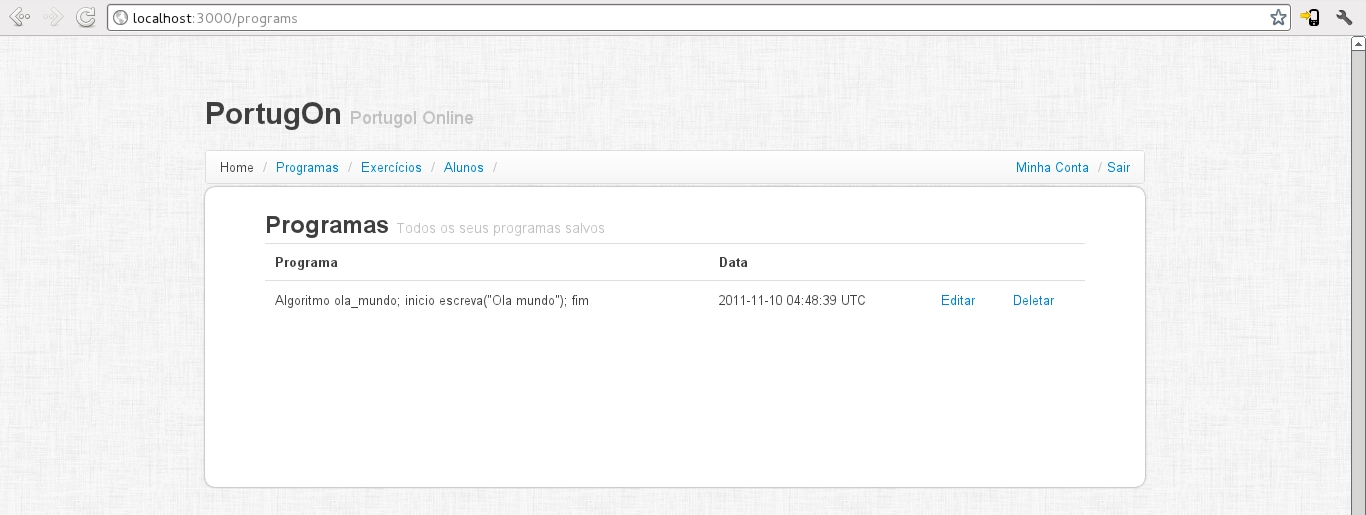
\includegraphics[scale=0.35]{imagens/tela5.jpg}
 \caption{P�gina Programas. Lista os programas j� efetuados pelo usu�rio}
\end{figure}

Caso o usu�rio ao realizar seu cadastro tenha escolhido o seu v�nculo como 'Professor', este ter� em sua p�gina o menu
'Exerc�cios'. Ao acessar tal menu, o usu�rio ser� capaz de criar um exerc�cio � ser aplicado e tamb�m, listar todos
os seus exerc�cios j� criados (figura 4.8). As oper��es de editar e excluir podem tamb�m serem utilizadas nessa se��o.

\begin{figure}[!htb]
 \centering
 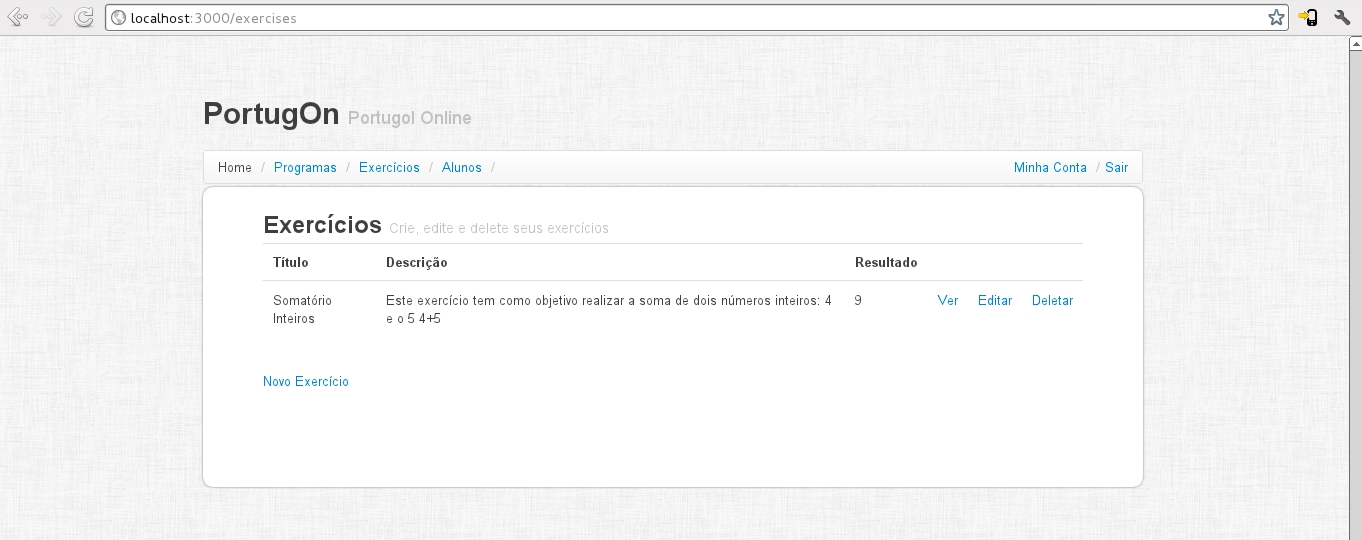
\includegraphics[scale=0.35]{imagens/tela6.jpg}
 \caption{P�gina Exerc�cios. Lista os exerc�cios criados pelo usu�rio}
\end{figure}

Se o usu�rio for do tipo 'Professor', aparecer� tamb�m no seu menu, o link 'Alunos'. Ao acessar este link o usu�rio
ir� para a p�gina respons�vel por listar os alunos atrelados aquele professor. Ser� poss�vel tamb�m cadastrar
um novo aluno, bem como excluir os j� existentes (figura 4.9). O usu�rio pode tamb�m, clicar nos exerc�cios de cada
aluno para poder ver a resposta do aluno para o determinado exerc�cio.

\begin{figure}[!htb]
 \centering
 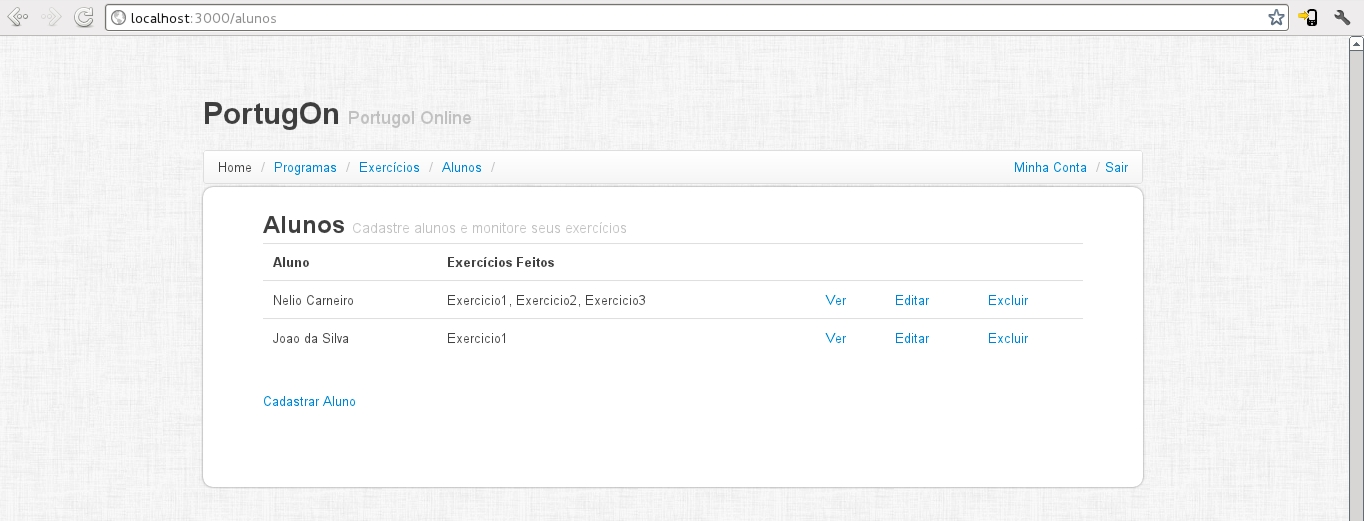
\includegraphics[scale=0.35]{imagens/tela7.jpg}
 \caption{P�gina Alunos. Lista os alunos criados pelo usu�rio}
\end{figure}

Ao encerrar as atividades no sistema, o usu�rio deve fazer o \textit{logout}, ou seja, encerrar sua sess�o no sistema.
Para isso, basta que ele clique em 'Sair', no menu ao lado direito.

\chapter{Teste e An�lise dos Resultados}
\input{quinto}



\newpage
%%%%%%%%%%%%%%%%%%%%
%%% BIBLIOGRAFIA %%%
%%%%%%%%%%%%%%%%%%%%
\pagestyle{empty}
\addcontentsline{toc}{chapter}{Refer�ncias}
\bibliographystyle{apalike}
\bibliography{Mono}




\label{ultimapagina}

\end{document}
